

\section{Proof Overview}\label{sec:overview}

\cref{alg:tsp} consists of two steps: sampling a tree whose marginals match $x$ (and hence has expected cost equal to $c(x)$), and then augmenting this with a minimum cost matching on the odd degree vertices of the tree. The goal of the current paper is to show that
the expected cost of the minimum cost matching on the odd degree vertices of the sampled tree is at most $(1/2-\eps)c(x)$. This is done by showing the existence of a cheap feasible $O$-join solution to \eqref{eq:tjoinlp}. Note that we merely need to prove the existence of a cheap $O$-join solution. The actual optimal $O$-join solution can be found in polynomial time.

First, note that if we only wanted to get an $O$-join solution of value at most $c(x)/2$, to \hyperlink{tar:satisfy}{satisfy} all cuts, it is enough to set $y_e := 0.5 x_e$ for each edge\footnote{This is because $x$ satisfies $x(\delta(S))\ge 2$ for all $S$, whereas $y$ must satisfy $y(\delta(S))\ge 1$ just for those cuts that have odd intersection with the tree $T$.} \cite{Wol80}. Now notice that if all of the near min cuts of $x$ containing $e$ are even, then we can reduce $y_e$ strictly below $0.5 x_e$.
The difficulty in implementing this approach comes from the fact that a high cost edge can be on many near min cuts and it may be exceedingly unlikely that {\em all} of these cuts will be even simultaneously. The idea in \cite{KKO21} is to initialize $y_e:= 0.5 x_e$ and then modify it by adding to it a random\footnote{where the randomness comes from the random sampling of the tree}  {\em slack vector} $s:E\to\R$: For each edge $e$, when  certain special (few) $\eta$-near-mincuts that $e$ is on are even in the tree, $s_e$ is set to  $-x_e \decrease$ where $\decrease\approx \eta/4$  chosen  in the proof of \cref{thm:main}; for other cuts that contain $e$, whenever they are odd, the slack of {\em other} edges on that cut is increased to satisfy them (i.e., maintain feasibility of $y$ for that cut). The bulk of the effort was to show that this can be done while guaranteeing that $\E{s_e}<-\eps x_e$ for some $\eps>0$, and therefore
$\E{y_e} = 0.5 x_e + \E{s_e} < (0.5 - \epsilon) x_e$.

To help the reader understand both the big picture as well as the ideas and contribution of the current paper, it is useful to first review in a bit more detail the approach taken in \cite{KKO21}. Let $\cN_\eta$ be the set of all $\eta$-near min cuts of $x$.
 A key idea there was to partition $\cN_\eta$ into three types: a set of near min cuts $\cH$ that form a {\em hierarchy} (which is a laminar family of  cuts), a set of cuts $\cN_{\eta,1}$ that are "crossed on one side" and a set of  cuts  $\cN_{\eta,2}$ that are "crossed on both sides"\footnote{ We will explain the terms in quotes shortly. Also, see \cref{defn:crossedonetwo}.}. \cite{KKO21} showed that if we \text{only} need to satisfy the $O$-Join constraints coming from $\cH$, then we can find such a vector $s$.
 
 %The negative slack component of $s_e$ (and hence the reduction in the cost of the min-cost matching relative to $0.5c(x)$) comes from considering only the cuts in the hierarchy and ensures that $O$-Join constraints for cuts in $\cH$ are satisfied even in the presence of this negative slack.  
%The event that certain cuts in $\cH$ are even in the tree is used to set $s_e$ to $-O(\eta) x_e$. However, as mentioned above, this may result in other cuts not being satisfied. In particular, if some cuts in $\cC_2$ are odd in the tree, but have some negative $s_e$ values, they
However, this vector $s$ (which is negative in expectation) might "break" O-join constraints on cuts that are {\em not} in the hierarchy (i.e., cuts in $\cN_{\eta,1}$ and  $\cN_{\eta,2}$). To resolve this, \cite{KKO21} showed how a negligible {\em increase} in the slack of certain edges (a  slack component they called $s^*$)  can be used to restore the feasibility of the O-join solution on \textit{all} cuts, including those that are not in the hierarchy.  See \cref{sec:hierarchy} for more on this.

Concretely,
because the cuts in $\cN_{\eta,2}$ have a rather complex structure,  to simplify their handling, \cite{KKO21} changed the plan: Instead of starting with $y_e = 0.5x_e$, they started with $y_e = (x_e + OPT_e)/2$, where $OPT_e$ is an indicator for edge $e$ being in the optimal integral TSP solution. They then constructed slack vectors relative to the near min cuts of $(OPT + x)/2$. The advantage of doing so is that it guarantees that all near mincuts correspond to intervals of vertices along the optimal cycle, {\em greatly} simplifying the structure of the family of near min cuts under consideration. Slack on the edges in the optimal cycle was then used to handle the cuts in $\cN_{\eta,1}$ and $\cN_{\eta,2}$. 

Unfortunately, this meant that the bound on the expected cost of the minimum cost matching from \cite{KKO21} is
at most $(1/2-\epsilon)((c(x) + c(OPT))/2$, which is insufficient to prove that the integrality gap of the LP is strictly below 3/2.

In the present paper, we return to the plan of initializing $y_e := 0.5 x_e$ and then construct a slack vector for each edge with the desired properties.  Our starting point is the {\em polygon decomposition}  $\mathcal D$ of the $\eta$-near min cuts of $x$~\cite{BG08}\footnote{See \cref{sec:polyrep} for a formal introduction to polygons. In particular, a reader unfamiliar with polygons will likely need to read \cref{sec:polybasics} to understand this section, though we provide a very brief overview now and again in \cref{sec:noinside}.}. 
%This decomposition is analogous to the cactus representation for the family of min-cuts, where the analogue of a cycle in a cactus is a polygon in  $\mathcal D$. 
As stated previously, a polygon\footnote{\ One difference between a cycle on $m$ nodes and a polygon with $m$  "outside atoms" is that  in a cycle all of the $m \choose 2$ simple cuts are min-cuts, whereas in a polygon only some of the $m \choose 2 $ simple cuts are $\eta$-near min cuts. Indeed a cycle is the "simplest" kind of polygon. Another major difference is that polygons may also have "inside" atoms. See \cref{sec:polyrep}.} is a connected component of crossing $2 + \eta$ near minimum cuts, where two cuts are connected if they cross each other.  It turns out that the way the polygon representation  $\mathcal D$ is constructed, each cut in $\cN_{\eta,2}$ is  in exactly one polygon, and each edge on such a cut will have its slack increase in at most one polygon. %\footnote{ However, an edge may be in $\delta(S)$ for multiple cuts in $\cC_2$ within that one polygon.}. 
Thus, cuts  in $\cN_{\eta,2}$ can be handled independently for each polygon. 
%We first show that 
%
%As discussed in Section ??, this allows us to partition the cuts into two sets, a hierarchy $\cH$, which is a laminar family of cuts and a set of cuts $C_2(\eta)$, where
%$$\cC = \cup _{\text{polygons }P\in \mathcal D}\{C\text{ near min cut in } P ~| ~C \text{ crossed on both sides}\}.$$

The main result of this paper is to show how to handle the cuts in $\cN_{\eta,2}$ (polygon by polygon) without resorting to the use of the OPT vector. Specifically, we prove the following: 
 \begin{theorem}[Informal main theorem]\label{thm:informalmain}
For any connected component $\cC$ of $\cN_\eta$ (i.e. a polygon),  let $\cC_2$ be the cuts in $\cC$ that are crossed on both sides. For any $\alpha>0$, there is a vector $s^*: E \rightarrow  R$ depending on $T$  s.t. 
\begin{enumerate}
\item[(i)] $\forall e \in E$, $s_e^*  \ge 0$;
\item[(ii)] $\E{s^*_e} = O(\eta \alpha x_e)$, where the expectation is over the choice of tree $T$.	
\item[(iii)] If $S\in \cC_2$ is a cut such that $\delta(S)_T$ is odd, then $s^*_T(\delta(S)) := \sum_{e \in \delta(S)} s^*_e \ge \alpha(1-\eta)$.
\end{enumerate}
 
\end{theorem}


Once cuts in $\cN_{\eta,2}$ are handled, the remaining cut structure becomes significantly simpler in that the polygons start to look very much like cycles: they contain only "outside atoms"\footnote{See \cref{sec:polybasics}.} and the fractional mass $x(a_i, a_{i+1})$ between adjacent atoms is $1\pm \Theta (\eta)$ ~\cite{KKO21}. This enables us, with minor modification to the way in which cuts crossed on one side are handled (see \cref{thm:crossed-one-side}), to adapt one of the main results in \cite{KKO21}.
\begin{restatable}[Informal Theorem adapted from \cref{thm:crossed-one-side} and \cref{thm:payment-main}]{theorem}{informalhierarchy}
\label{thm:hierarchyKKO}
Given a family $\cN_{\eta,\leq 1}$ of near-min cuts containing {\bf  no} cuts crossed on both sides, for any $\decrease>0$, there is a vector $s: E \rightarrow \R$
 depending on $T$ such that	\begin{enumerate}
\item [(i)] $\forall e \in E$, $s_e  \ge -\decrease  x_e$ %and $s_e^* \ge 0$ (both with probability 1)
\item [(ii)] $\E{s_e} < -\epsilon \decrease x_e$ for some absolute constant $\epsilon > 0$, independent of $\eta$, %and $\E{s^*_e} = O(\eta^2 x_e)$ 
where the expectations are over the choice of $T$.
\item [(iii)] If $S \in \cN_{\eta,\leq 1}$ is a cut such that $\delta(S)_T$ is odd, then $s_T(\delta(S)) = \sum_{e \in \delta(S)} s_e \ge 0$.
\end{enumerate}
\end{restatable}
Note that \cref{thm:payment-main} (used to prove the above theorem) crucially relies on the fact that the tree is sampled from a max-entropy distribution, whereas \cref{thm:informalmain} does not.

Before we explain the ideas underlying the proof of \cref{thm:informalmain}, we quickly show how by setting
$$y_e(T):= 0.5 x_e + s^*_e+ s_e\quad\forall e,$$
these two theorems together imply  the main result of this paper.

First, we show that $\E{c(y) }\le c(x) (0.5-\epsilon)$ 
To see this, observe that  \cref{thm:informalmain}(ii)  together with 
\cref{thm:hierarchyKKO}(ii) imply  that for every edge $e \in E$,
$$\E{y_e} =  0.5x_e + \E{s_e} + \E{s^*_e}\\
 \le x_e \left(0.5  + O(\eta\alpha) - \epsilon \decrease\right)  \le x_e \left(0.5 - \eta\eps'\right),$$
for $\alpha,\beta$ as chosen below and $\eta$ sufficiently smaller than $\epsilon$. 
Summing over all edges, this gives
$$\E{c(y)} \le \left(\frac{1}{2} - \epsilon'\right)c(x).$$
Note that since $s_e^*$ is always nonnegative, it does not help us in our quest to reduce $y_e$ strictly below $0.5 x_e$. That reduction comes only from $s_e$ being negative. Indeed, the raison d'etre  of the slack vector $s^*$ is to repair the feasibility of cuts which are odd in the tree but which have $s_e$ negative on some edges in $\delta(S)$. This is why it is crucial that $\E{s_e}$ is much smaller than $-\E{s_e^*}$. 

Next, we show that $y(T)$ is feasible for every tree $T$. For this, we need to consider three types of cuts: 

\paragraph{Case 1:} $\delta(S)_T$ is odd and $x(\delta(S)) > 2 + \eta$. Since $s^*_T(\delta(S))\ge 0$ and $s_T(\delta(S)) \ge -\decrease x(\delta(S)$, we have
$$ y_T(\delta(S)) = 0.5x(\delta(S))+ s^*_T(\delta(S)) + s_T(\delta(S)) \ge (0.5 - \decrease)x(\delta(S))\ge (0.5 - \decrease)(2 + \eta) \ge 1,$$
for $\decrease \approx \eta/4$.

\paragraph{Case 2:}$\delta(S)_T$ is odd, $S\in \cN_{\eta,\leq 1}$. In this case $s_T(\delta(S)),s^*_T(\delta(S))\ge 0$ so $y_T(\delta(S) \ge 0.5 x(\delta(S)) \ge 1.$
%\Shayan{Change $S$ odd to $\delta(S)_T$ odd?}
\paragraph{Case 3:}$\delta(S)_T$ is odd, $x(\delta(S)) \le  2 + \eta$, and $S\in\cN_{\eta,2}$. In this case, 
 $s^*_T(\delta(S))\ge  \alpha(1-\eta)$ and $s_T(\delta(S)) \ge -\decrease x(\delta(S))$, so we have
$$ y_T(\delta(S)) = 0.5 x(\delta(S))+ s^*_T(\delta(S) + s_T(\delta(S)) \ge (0.5 - \decrease)x(\delta(S)) + \alpha(1-\eta) \ge %(0.5 - \eta/8)2 + \eta/4\ge 
1,$$
for $\alpha\approx 2\decrease$ using $x(\delta(S))\ge 2$.

\vspace{0.2in}
\begin{figure}[htb!]\centering
	\begin{tikzpicture}
	\pattern[pattern=north east lines, pattern color=blue!35] (228:3) -- +(1,0) -- (180:3) arc (180:228:3); 
	\pattern [pattern=north east lines, pattern color=purple!35] (312:3) -- +(-1,0) -- (360:3) arc (360:276:3);
		\fill [color=purple!15] (276:3) -- (294:2.4) -- (312:3)  arc (312:276:3); 
		\fill [color=blue!15] (228:3) -- (246:2.4) -- (264:3) arc (264:228:3);
		\foreach \i/\l in {0/0, 180/15, 192/16, 204/17, 216/18, 228/19, 240/20, 252/21, 264/22, 276/23, 288/24, 300/25, 312/26, 324/27, 336/28, 348/29}
			\node [fill, circle, inner sep=0.5mm] at (\i:3) (p_\l) {};
		\foreach \i/\j in { 15/16, 16/17, 17/18, 18/19, 19/20, 20/21, 21/22, 22/23, 23/24, 24/25, 25/26, 26/27, 27/28, 28/29, 29/0}
			\path (p_\i) edge (p_\j);	
		\foreach \i/\l in {19/l, 26/r}
			\node at (\i*12:3.4) () {\footnotesize $p_\l$};	
		\path [color=green,line width=1.2pt] (p_19) edge node [above] {$S$} (p_26);
		\node [color=blue] at (184:2.3) (){$S_L$};
		\node [color=red] at (356:2.3) () {$S_R$};
		\path [color=blue,line width=1.2pt] (p_22) edge  (p_15);
		\path [color=purple,line width=1.2pt] (p_23) edge  (p_0);
		\node [color=orange] at (204:3.7) () {\small $S_L\smallsetminus S$};
		\node [color=blue] at (245:3.4) (){\small $S^{\cap L}$};
		\node [color=red] at (295:3.4) (){\small $S^{\cap R}$};
		\node [color=green] at (335:3.7) (){\small $S_R\smallsetminus S$};
		\foreach \i/\c in {186/orange, 198/orange, 210/orange, 222/orange, 234/blue, 246/blue, 258/blue, 282/red, 294/red, 306/red, 318/green, 330/green, 342/green, 356/green}
			\node [circle,fill,inner sep=0.8mm,color=\c] at (\i:3) () {};  
		\node at (295:2.9) (b1) {}; \node at (340:2.9) (b2) {};
		\node at (245:2.9) (a1) {}; \node at (200:2.9) (a2) {};
		\path [color=red,->,line width=1.3pt] (b1) edge [bend left=90] (b2) ;
		\path [color=blue,->,line width=1.3pt](a1) edge [bend right=90] (a2);
	\end{tikzpicture}
\caption{\footnotesize (Note that to simplify the pictures, we usually draw a polygon as a circle.)  The figure shows a cut $S$ that is crossed on both sides. The cut $S$ consists of all atoms below the green line. The cut $S_R$ is the cut crossing $S$ on the right which minimizes the number of outside atoms in the intersection, i.e., it minimizes the number of red atoms. Similarly, $S_L$ crosses $S$ on the left and minimizes the number of blue atoms. While not shown in the picture, it's possible for the red and blue atoms to overlap. ($S_R$ might cross $S_L$.) Edges between red atoms and green atoms are in $E^\rightarrow (S)$ and edges between blue atoms and orange atoms are in $E^\leftarrow(S)$. Edges in $E^\circ(S)$ are all remaining edges in $\delta(S)$. \cref{claim:C2evenwhp} shows that with probability $1 - O(\eta)$, in the randomly sampled tree $T$, there is exactly one (red,green) edge (i.e., $B^\rightarrow(S)$ does not occur) and exactly one (blue, orange) edge (i.e., $B^\leftarrow(S)$ does not occur)  and those are the only edges in $\delta(S) \cap T$ (i.e., also  $B^\circ(S)$ does not occur).}
 %tree that arein Since intersections and differences of $\eta$-near min cuts are $2\eta$-near min cuts the  sets $S^{\cap R}$ and $S_R \setminus S$ are $2\eta$-near min cuts, so by \cref{lem:treeoneedge}, with probability $1-O(\eta)$ there is exactly one edge in the tree between the dark red region on the light red region (respectively dark blue region and light blue region), and similarly  with probability $1-O(\eta)$ those are the only two edges in $\delta(S) \cap T$.
	\label{fig:S-SR-SL}
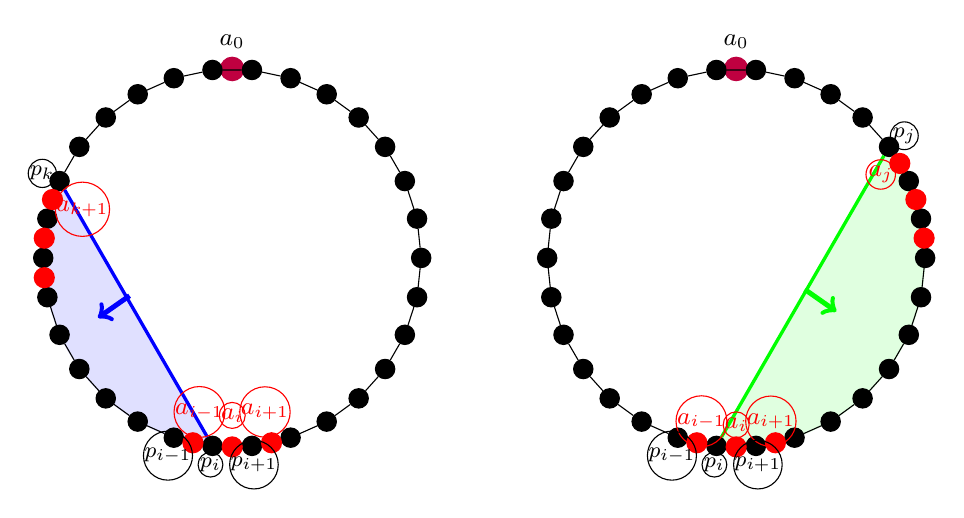
\begin{tikzpicture}[scale=0.8]
		\fill [color=blue!12] (264:3) arc (264:156:3);
		\node [inner sep=3, fill, circle, color=purple, label={[yshift=0]\small $a_0$}] at (90:3) (){};
		\foreach \i/\l in {0/0, 12/1, 24/2, 36/3, 48/4, 60/5, 72/6, 84/7, 96/8, 108/9, 120/10, 132/11, 144/12, 156/13, 168/14, 180/15, 192/16, 204/17, 216/18, 228/19, 240/20, 252/21, 264/22, 276/23, 288/24, 300/25, 312/26, 324/27, 336/28, 348/29}
			\node [fill, circle, inner sep=0.5mm] at (\i:3) (p_\l) {};
			\path [line width=1.2pt,color=blue] (p_22) edge (p_13);
			\draw [line width=1.8,color=blue,->] (-1.63,-0.6) -- +(-0.5,-0.35);
		\foreach \i/\j in {0/1, 1/2, 2/3, 3/4, 4/5, 5/6, 6/7, 7/8, 8/9, 9/10, 10/11, 11/12, 12/13, 13/14, 14/15, 15/16, 16/17, 17/18, 18/19, 19/20, 20/21, 21/22, 22/23, 23/24, 24/25, 25/26, 26/27, 27/28, 28/29, 29/0}
			\path (p_\i) edge (p_\j);
		\foreach \i/\l in {258, 270, 282,  162, 174, 186}
			\node [fill,red,circle,inner sep=0.9mm] at (\i:3) (){}; 
		\foreach \i/\l in {258/i-1, 270/i, 282/i+1, 162/k+1}
			\node [color=red] at (\i:2.5) () {\small $a_{\l}$}	;
		
		\foreach \i/\l in {252/i-1, 264/i, 276/i+1, 156/k}
			\node  at (\i:3.3) () {\footnotesize $p_{\l}$};

		\begin{scope}[xshift=8cm]
			\fill [color=green!12] (264:3) arc (264:396:3);
			\node [inner sep=3, fill, circle, color=purple, label={[yshift=0]\small $a_0$}] at (90:3) (){};
		\foreach \i/\l in {0/0, 12/1, 24/2, 36/3, 48/4, 60/5, 72/6, 84/7, 96/8, 108/9, 120/10, 132/11, 144/12, 156/13, 168/14, 180/15, 192/16, 204/17, 216/18, 228/19, 240/20, 252/21, 264/22, 276/23, 288/24, 300/25, 312/26, 324/27, 336/28, 348/29}
			\node [fill, circle, inner sep=0.5mm] at (\i:3) (p_\l) {};
			\path [line width=1.2pt,color=green] (p_22) edge (p_3);
			\draw [line width=1.8,color=green,->] (1.09,-0.5) -- +(0.5,-0.35);
		\foreach \i/\j in {0/1, 1/2, 2/3, 3/4, 4/5, 5/6, 6/7, 7/8, 8/9, 9/10, 10/11, 11/12, 12/13, 13/14, 14/15, 15/16, 16/17, 17/18, 18/19, 19/20, 20/21, 21/22, 22/23, 23/24, 24/25, 25/26, 26/27, 27/28, 28/29, 29/0}
			\path (p_\i) edge (p_\j);
		\foreach \i/\l in {258, 270, 282, 30, 18, 6}
			\node [fill,red,circle,inner sep=0.9mm] at (\i:3) (){}; 
		\foreach \i/\l in {258/i-1, 270/i, 282/i+1, 30/j}
			\node [color=red] at (\i:2.65) () {\small $a_{\l}$}	;
		
		\foreach \i/\l in {252/i-1, 264/i, 276/i+1, 36/j}
			\node  at (\i:3.3) () {\footnotesize $p_{\l}$};
	
		\end{scope}

	\end{tikzpicture}
\caption{\small Of all cuts crossed on both sides, $L(p_i)$, the blue set, extends farthest to the left from $p_i$. Similarly, $R(p_i)$, the green set, is the one that extends farthest to the right from $p_i$.  (For reference when we later include inside atoms: if the root is not an outside atom, $L(p_i)$ can wrap around past $a_0$ and there may be atoms in the interior of the blue region, aka inside atoms. However, the outside atoms of $L(p_i)\cup R(p_i)$ form a contiguous interval around the cycle and don't include all outside atoms. Even in the case in which the root is not an outside atom, the shaded region is the side of the diagonal which does not contain the root.) %it cannot cross  $L(p_i)$ of the "non"-$p_i$ side, as that would violate \autoref{obs:Ocross}.)
}
	\label{fig:LpRp}
\end{figure}

\begin{figure}[htb]\centering
	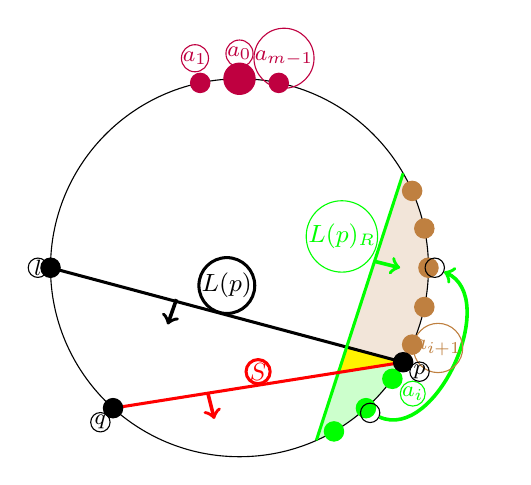
\begin{tikzpicture}[scale=0.8]
		\fill [color=yellow] (330:3) -- ++(-1.07,-0.19) -- +(0.2,0.45);
		\fill [color=green!20] (294:3) -- (330:3)+(-1.07,-0.19) -- (330:3) arc (330:294:3);
		\fill [color=brown!20] (330:3) -- (330:3)+(-0.87,0.26) -- (390:3) arc (390:330:3);
		\draw (0,0) circle (3);
		\foreach \i/\c in {78/purple, 90/purple, 102/purple, 324/green, 312/green, 300/green, 336/brown, 348/brown, 0/brown, 12/brown, 24/brown}{
			\node [circle,inner sep=2,color=\c,fill] at (\i:3) () {};
			}
		\node at (312:3.1) (a){}; \node at (0:3.1) (b) {};
		\path [color=green,->,line width=1.3pt](a) edge [bend right=90] (b);
		\foreach \i/\c/\l in {78/purple/m-1, 90/purple/0, 102/purple/1, 324/green/i, 338/brown/i+1}
			\node [color=\c] at (\i:3.4) () {\footnotesize $a_{\l}$};
		\node [circle,inner sep=4,color=purple,fill] at (90:3) (){};
		\draw [color=black,line width=1.1pt] (330:3) -- node [above] {\small $L(p)$} (180:3);
		\node [circle,fill,inner sep=2] at (180:3) () {};
		\node at (180:3.2) () {\footnotesize $l$};
		\draw [color=green, line width=1.1pt] (294:3) --  (30:3);
		\node [green] at (17:1.7) () {\small $L(p)_R$};
		\draw [color=red,line width=1.1pt] (330:3) -- node [above] {\small $S$} (228:3);
		\foreach \i/\l in {228/q,330/p}{
			\node [circle,fill,inner sep=1.5] at (\i:3) () {};
			\node at (\i:3.3) () {\footnotesize$\l$};
		}
		\draw [color=black,->,line width=1.3pt] (-1,-0.5) -- +(-.14,-0.4);
		\draw[color=red,->,line width=1.3pt] (-0.5,-2) -- +(0.1,-.4);
		\draw[color=green,line width=1.3pt,->] (2.15,0.1) -- +(0.4,-0.1);
	\end{tikzpicture}
	\caption{\footnotesize  Since $S$ is crossed on the right and any cut that crosses $S$ on the right also crosses $L(p)$ on the right,  the cut $S_R$, which contains the fewest number of atoms in $S$ (green atoms), is the same as $L(p)_R$. The edges in  $E^\rightarrow(L(p))= E^\rightarrow(S)$ are those that go between green atoms and brown atoms. Note also that any edge in $\delta(S)$ with one endpoint to the right of $p$  that is {\em not} in $E^\rightarrow(L(p))$ is in  $E^\circ(L(p))$. (It can't be in $E^\leftarrow(L(p))$ since those edges have one endpoint to the left of $l$.) 
	Note also that since the green + yellow region as well as the brown region are each the difference of two crossing $\eta$ near min cuts, each is a $2\eta$ near min cut. So by \autoref{lem:sub-NMC-shared}, the fraction of edges with one endpoint in each of these regions is $1-O(\eta)$. (To extend this to the case where polygon $P$ may have inside atoms we show that there are no atoms in the yellow region see \cref{lem:samerightEPsameedgeset}, or \cref{thm:halfplanes} for a more general statement.)
	}
	\label{fig:ErL=ErS}
\end{figure}




\begin{figure}[htb]\centering
	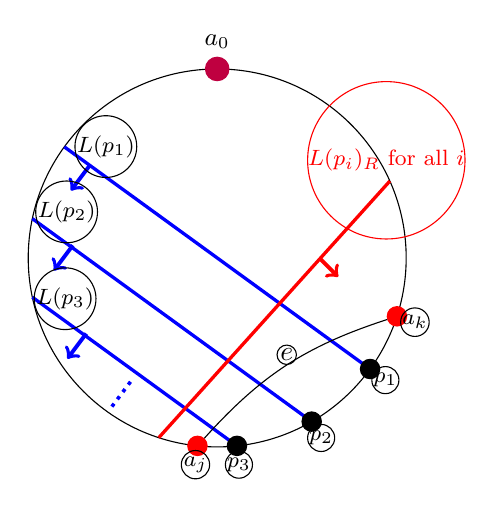
\begin{tikzpicture}[scale=0.8]
		\draw (0,0) circle (3);
		\node [circle,fill,purple,inner sep=3,label={[yshift=0cm]\small $a_0$}] at(90:3)() {};
		\draw [color=blue,line width=1.2pt] (324:3) -- (144:3)
		(300:3) -- (168:3) (276:3) -- (192:3);
		\draw[color=blue,line width=1.3pt,dotted] (235:2.4)-- +(-0.3,-0.4);
		\draw[color=red,line width=1.2pt] (252:3) -- (24:3);
		\foreach \i/\l in {324/1, 300/2, 276/3}{
			\node [fill,circle,inner sep=2] at (\i:3) (){ };
			\node at (\i:3.3) () {\footnotesize $p_{\l}$};
		}
		\node [circle,color=red,fill,inner sep=2] at (264:3) (a) {};
		\node [circle,color=red,fill,inner sep=2] at (342:3) (b) {} edge [bend right=15] node [above] {$e$} (a);
		\node at (264:3.3) () {\footnotesize $a_j$};
		\node at (342:3.3) () {\footnotesize $a_k$};		
		\draw [color=blue,line width=1.4pt,->] (144:2.5) -- +(-0.3,-0.4);
		\draw [color=blue,line width=1.4pt,->] (175:2.3) -- +(-0.3,-0.4);
		\draw [color=blue,line width=1.4pt,->] (210:2.4) -- +(-0.3,-0.4);
		\draw[color=red,line width=1.4pt,->] (0:1.62) -- +(0.3,-0.3);
		\node [color=red]at (30:3.1) () {\footnotesize $L(p_i)_R$ for all $i$};
		\foreach \i/\l in {135/1, 163/2, 195/3}
			\node at (\i:2.5) () {\footnotesize $L(p_{\l})$};
	\end{tikzpicture}
	\caption{\small Edge $e= \{a_j,a_k\}$ is in $E^\rightarrow(L(p_i))$ for all $i$.}
	\label{fig:einmanyL(p)}
\end{figure}


\begin{figure}[htb]
\centering
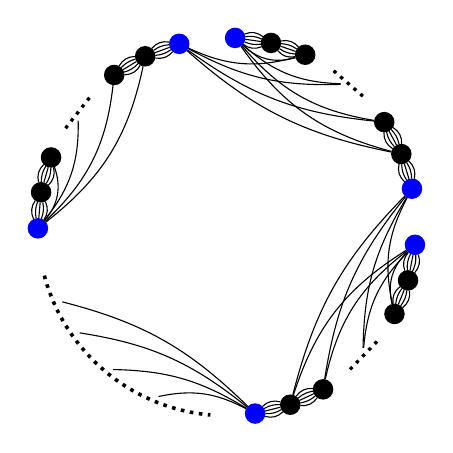
\begin{tikzpicture}[scale=0.8]
\tikzstyle{every node} = [inner sep=0,minimum size=7,draw,fill=none,circle];
\foreach \a in {0, 1, 2}{
\begin{scope}[rotate=93*\a]
\foreach \i/\l/\c in {0.5/0/blue, 1.5/1/black, 2.5/2/black,  5.4/4/black,6.4/5/black,7.4/6/blue}{
	\node at (-\i*11:3) [color=\c,fill] (\a_\l) {};
}
\node at (-4*11:3) [draw=none] (\a_3) {};
\foreach \i/\j in {0/1, 1/2, 4/5, 5/6}{
	\path (\a_\i) edge  (\a_\j) (\a_\i) edge [bend left=15] (\a_\j);\path (\a_\i) edge [bend right=15] (\a_\j);
	\path (\a_\i) edge [bend left=30] (\a_\j);\path (\a_\i) edge [bend right=30] (\a_\j);
}
\path (\a_0) edge [bend right=30](\a_2);
\foreach \i in {3,...,5}{
	\path (\a_0) edge [bend right=20](\a_\i);}
\draw [dotted,line width=1.2] (-3.4*11:3) -- (-4.6*11:3);
%\draw [decorate, decoration={brace, segment length=40mm, amplitude=3mm}] (-1*11:3.5) arc (-1*11:-8*11:3.5);
%\curlybrace[color=blue,thick]{-1*11}{-8*11}{3.5}
\end{scope}
}
\begin{scope}[rotate=91*3]
\foreach \i/\l/\c in {0.5/0, 1.5/1, 2.5/2,  4/3, 5.4/4, 6.4/5,7.4/6}{
	\node at (-\i*11:3) [draw=none] (3_\l) {};
}
\end{scope}
\foreach \a/\b in {1/0,2/1, 0/3}{
	\path (\a_6) edge [bend right=20](\b_2)  (\a_6) edge [bend right=15] (\b_3)
	(\a_6) edge [bend right=15](\b_4)
	(\a_6) edge [bend right=15] (\b_5);
}
\draw [dotted, line width=1.3] (195:3) arc (195:265:3);
\end{tikzpicture}
\caption{\small Suppose that there are exactly $1/\eta$ (black) vertices between any two vertices in the above figure, where each edge has fractional value $\eta$.  Also, any two consecutive vertices (if both of them are not blue) have exactly $1/\eta$ parallel edges between them. Then, it is easy to check that the above graph is fractionally $2$ edge connected.
Furthermore, the set of $2+O(\eta)$-near minimum cuts comprises a single connected component and every vertex will become an (outside) atom of the corresponding polygon. This is because every diagonal which separates two blue vertices on both sides is a near min cut. In addition, every interval with $O(1)$ many consecutive vertices where at most one of vertex is blue is also a near mincut. In such a case, for every pair of adjacent blue vertices, we have $E(a_i, a_{i+1}) = \emptyset$. }
\label{fig:nearmincutbadexample}
\end{figure}


\begin{figure}[htb]\centering
	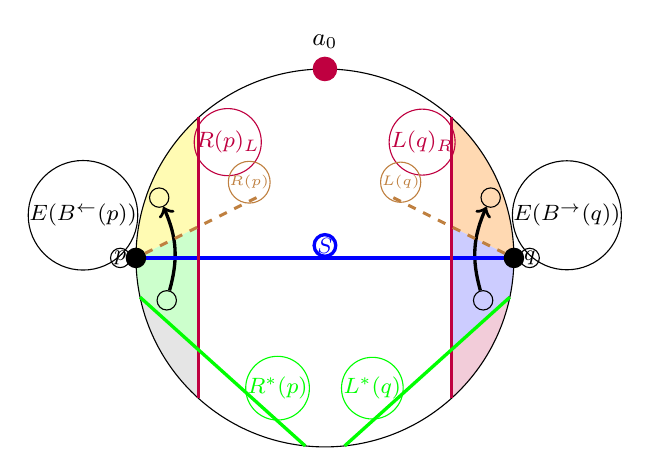
\begin{tikzpicture}[scale=0.8]
		\fill [color=gray!20](228:3) -- +(0,0.75)-- (192:3) arc (192:228:3);
		\fill [color=purple!20] (312:3) -- +(0,0.75) -- (-12:3) arc (348:312:3);
		\fill [color=yellow!30] (180:3) -- +(1,0.5) -- (132:3) arc (132:180:3);
		\fill [color=orange!30] (0:3) -- +(-1,0.5) -- (48:3) arc (48:0:3);
		\fill [color=green!20] (180:3) -- ++(1,0.5) -- +(0,-2) -- (192:3) arc (192:180:3);
		\fill [color=blue!20] (0:3) -- ++(-1,0.5) -- +(0,-2) -- (-12:3) arc (-12:0:3);
		\node at (195:2.6) (a1){}; \node at (160:2.8) (a2) {};
		\node at (-15:2.6) (b1) {};\node at (20:2.8) (b2){};
		\path [line width=1.2pt,->] (a1) edge [bend right=20] (a2);
		\path [line width=1.2pt,->] (b1) edge [bend left=20] (b2);
		\node at (10:3.9) () {\footnotesize $E(B^\rightarrow(q))$};
		\node at (170:3.9) () {\footnotesize $E(B^\leftarrow(p))$};
		\draw (0,0) circle (3);
		\node [circle,fill,purple,inner sep=3,label={[yshift=0cm]\small $a_0$}] at(90:3)() {};
		\draw [color=blue,line width=1.2pt] (0:3) -- node [above] {\footnotesize $S$} (180:3);
		\foreach \i/\c/\l in {180/black/p, 0/black/q}{
			\node [circle,inner sep=2,color=\c,fill] at (\i:3) (\l) {};
			\node at (\i:3.25) () {\footnotesize $\l$};
		}
		\draw [color=purple,line width=1.2pt] (132:3) --(228:3) (48:3) --(-48:3);
		\node[color=purple] at (130:2.4) () {\footnotesize$R(p)_L$};
		\node [color=purple] at (50:2.4) () {\footnotesize $L(q)_R$};
		\draw [color=brown,dashed,line width=1.1pt] (p) -- +(2,1) (q) -- +(-2,1);
		\node [color=brown]at (45:1.7) () {\tiny $L(q)$};
		\node [color=brown] at (135:1.7) () {\tiny $R(p)$};
		\draw [color=green,line width=1.2pt] (192:3) -- (264:3) (276:3) -- (-12:3);
		\node [color=green] at (250:2.2) () {\footnotesize $R^*(p)$};
		\node [color=green] at (290:2.2) () {\footnotesize $L^*(q)$};
	\end{tikzpicture}
	\caption{\small This figure illustrates the definitions in (\ref{defn:slackincrease}). The near min cut S contains all atoms below the blue line. $L(q)_R$ crosses $L(q)$ on the right and $R(p)_L$ crosses $R(p)$ on the left. $L(q)^{\cap R}$ is the set of atoms in the blue + pink region on the right. $L^*(q)$ is the near min cut crossing $L(q)^{\cap R}$ on the left that maximizes the number of outside atoms in the pink region. Similarly $R^*(p)$ is the near min cut crossing $R(p)^{\cap L}$ on the right that maximizes the number of outside atoms in the grey region. The edges in $E(B^\rightarrow (q))$ are those edges from the blue region to the orange region and the edges in $E(B^\leftarrow (p))$ are those edges from the green region to the yellow region. Note that the figure is misleading in that sets that are shown as disjoint here may not in fact be disjoint.}
	\label{fig:L*R*}
\end{figure}


\begin{figure}[htb]\centering
	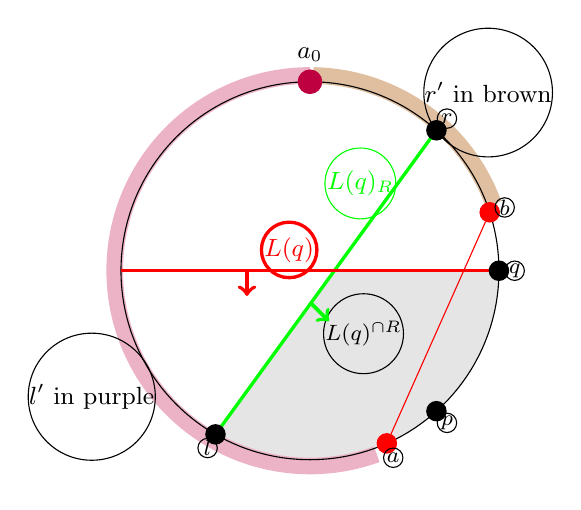
\begin{tikzpicture}[scale=0.8]
		\fill [color=gray!20] (240:3) -- (0.4,0) -- (0:3) arc (360:240:3);

		\draw [color=purple!30,line width=6pt] (90:3.1) arc  (90:290:3.1);
		\draw [color=brown!50,line width=6pt] (20:3.1) arc (20:89:3.1);
		\draw [color=green,line width=1.2pt] (240:3) -- (48:3);
		\node at (0.85,-1) () {\footnotesize $L(q)^{\cap R}$};
		\node [color=green] at(60:1.6) () {\small $L(q)_R$};
		\draw [line width=1.4pt,->,color=green] (0,-0.5) -- +(0.3,-0.3);
		\node at (45:4) () {\small \text{$r'$ in brown}};
		\node at (210:4) () {\small $l'$ in purple};
		\draw (0,0) circle (3);
		\node [circle,fill,purple,inner sep=3,label={[yshift=0cm]\small $a_0$}] at(90:3)() {};
		\draw [color=red,line width=1.2pt] (0:3) -- node [above left] {\small $L(q)$} (180:3);
		\draw [color=red,->,line width=1.4pt] (-1,0) -- +(0,-0.4);
		\foreach \i/\c/\l in {0/black/q, 312/black/p, 18/red/b, 294/red/a, 240/black/l, 48/black/r}{
			\node [circle,inner sep=2,fill,color=\c] at (\i:3) (\l) {};
			\node at (\i:3.25) () {\footnotesize $\l$};		
		}
		\path [color=red] (a) edge (b); 
	\end{tikzpicture}
	\caption{\small  Setup for proof of \cref{claim:atmost2sets}: Let $L(q)_R = (l,r)$ and $L(p)_R=(l',r')$ (where $l,r,l',r'$ are polygon points). The grey region is $L(q)^{\cap R}:= L(q) \cap L(q)_R$. Note that neither $L(p)$ or $L(p)_R$ are shown in this figure, since our proof in fact will need to argue about how these cuts are situated relative to those shown.  WLOG (as shown in the figure) $p$ is to the left of $q$. Now, for contradiction, suppose that $e=\{a,b\}\in E(B^\rightarrow(p))\cap E(B^\rightarrow(q))$. Then $a,b\in L(p)_R\cap L(q)_R$. So, in the above, since no cut contains $a_0$, it must be that $l'$ is to the left of $a$ and $r'$ is to the right of $b$.}
	\label{fig:locl'r'circ}
\end{figure}



	
\def\scale{0.7}
\begin{figure}[htb!]\centering
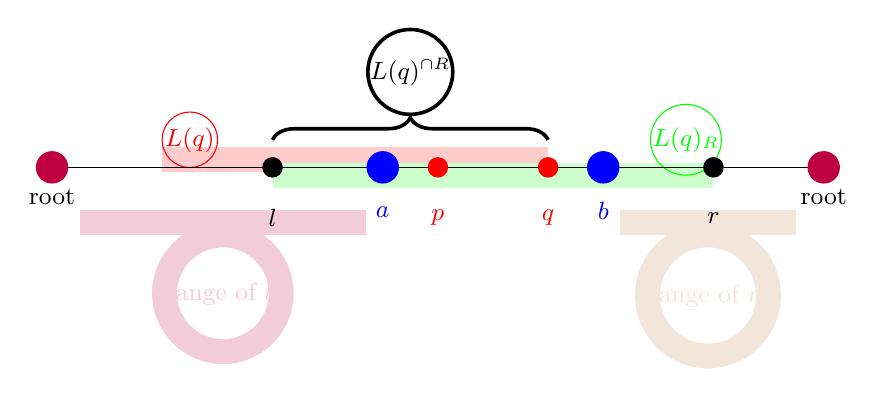
\begin{tikzpicture}[scale=\scale]
	\draw [decorate,line width=1.3pt, decoration = {brace,mirror,amplitude=8pt}] (9,0.5) --node [above=0.3cm] {\small $L(q)^{\cap R}$}  (4,0.5);
		\draw [color=red!20,line width=9pt]	(9,0.15) -- (2,0.15);
		\draw [color=green!20,line width=9pt] (12,-0.15) -- (4,-0.15);
		\draw [color=purple!20,line width=9pt] (5.7,-1) -- node [below] {\small range of $l'$}(0.5,-1);
		\draw [color=brown!20,line width=9pt] (10.3,-1) -- node [below] {\small range of $r'$}(13.5,-1);
		\node [color=red] at (2.5,0.5) () {\small $L(q)$};
		\node [color=green] at (11.5,0.5) () {\small $L(q)_R$};
		\draw [color=black] (0,0) -- (14,0);
		\foreach \i in {0, 14}
			\node [color=purple,inner sep=4,label={[yshift=-0.9cm]\small root},circle,fill] at (\i,0) () {};
		\foreach \i/\c/\l/\is in {4/black/l/2, 6/blue/a/4, 7/red/p/2, 9/red/q/2, 10/blue/b/4, 12/black/r/2}
			\node [fill,circle,inner sep=\is,label={[yshift=-0.9cm,color=\c]\small $\l$},color=\c] at (\i,0) () {};
	\end{tikzpicture}
	\caption{\small  Proof of \cref{claim:atmost2sets} continued: Because we are dealing with outside atoms only and no cuts contain the root $a_0$, we may as well visualize the polygon as a line (with wraparound) and each cut as an interval along the line.  The above figure repeats \cref{fig:locl'r'circ} when viewed as a line segment. }
	\label{fig:locl'r'}

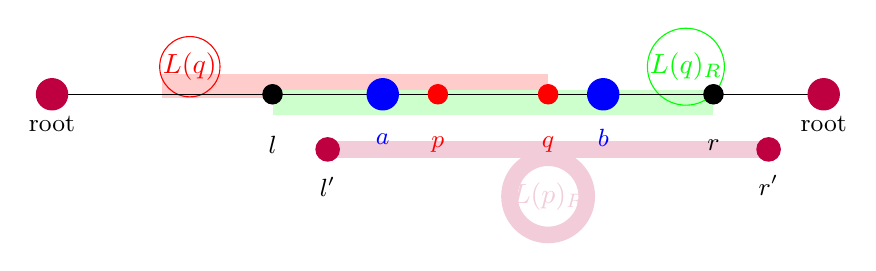
\begin{tikzpicture}[scale=\scale]
			\draw [color=red!20,line width=9pt]	(9,0.15) -- (2,0.15);
		\draw [color=green!20,line width=9pt] (12,-0.15) -- (4,-0.15);
		\draw [color=purple!20,line width=6pt] (5,-1) -- node [below] {$L(p)_R$}(13,-1);
		\foreach \i/\l in {5/l',13/r'}
			\node [circle,color=purple,fill,inner sep=3, label={[yshift=-0.8cm]\small$\l$}] at (\i,-1) () {};
%		\draw [color=brown!20,line width=9pt] (10.3,-1) -- node [below] {range of $r'$}(13.5,-1);
		\node [color=red] at (2.5,0.5) () {$L(q)$};
		\node [color=green] at (11.5,0.5) () {$L(q)_R$};
		\draw [color=black] (0,0) -- (14,0);
		\foreach \i in {0, 14}
			\node [color=purple,inner sep=4,label={[yshift=-0.9cm]\small root},circle,fill] at (\i,0) () {};
		\foreach \i/\c/\l/\is in {4/black/l/2, 6/blue/a/4, 7/red/p/2, 9/red/q/2, 10/blue/b/4, 12/black/r/2}
			\node [fill,circle,inner sep=\is,label={[yshift=-0.9cm,color=\c]\small $\l$},color=\c] at (\i,0) () {};
	\end{tikzpicture}
	\caption{\small  Claim: $l'$ can not be to the right of $l$. If it is, as in the figure above, then $L(p)_R$ crosses $L(q)$ on the right and has a smaller intersection with $L(q)$. Contradiction to choice of $L(q)_R$!}
	\label{fig:l'notR}
	
	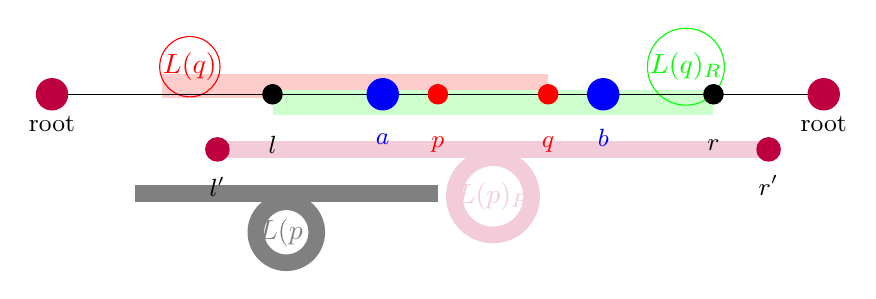
\begin{tikzpicture}[scale=\scale]
			\draw [color=red!20,line width=9pt]	(9,0.15) -- (2,0.15);
		\draw [color=green!20,line width=9pt] (12,-0.15) -- (4,-0.15);
		\draw [color=purple!20,line width=6pt] (3,-1) -- node [below] {$L(p)_R$}(13,-1);
		\draw [color=gray,line width=6pt] (7,-1.8) -- node[below] {$L(p)$} (1.5,-1.8);
		\foreach \i/\l in {3/l',13/r'}
			\node [circle,color=purple,fill,inner sep=3, label={[yshift=-0.8cm]\small$\l$}] at (\i,-1) () {};
%		\draw [color=brown!20,line width=9pt] (10.3,-1) -- node [below] {range of $r'$}(13.5,-1);
		\node [color=red] at (2.5,0.5) () {$L(q)$};
		\node [color=green] at (11.5,0.5) () {$L(q)_R$};
		\draw [color=black] (0,0) -- (14,0);
		\foreach \i in {0, 14}
			\node [color=purple,inner sep=4,label={[yshift=-0.9cm]\small root},circle,fill] at (\i,0) () {};
		\foreach \i/\c/\l/\is in {4/black/l/2, 6/blue/a/4, 7/red/p/2, 9/red/q/2, 10/blue/b/4, 12/black/r/2}
			\node [fill,circle,inner sep=\is,label={[yshift=-0.9cm,color=\c]\small $\l$},color=\c] at (\i,0) () {};
	\end{tikzpicture}
	\caption{\small Claim: $l'$ can not be to the left of $l$. If so, as in the figure above, then $L(q)_R$ crosses $L(p)$ on the right and has a smaller intersection with $L(p)$. Contradiction to choice of $L(p)_R$! Therefore $l'=l$.}
	\label{fig:l'notL}
	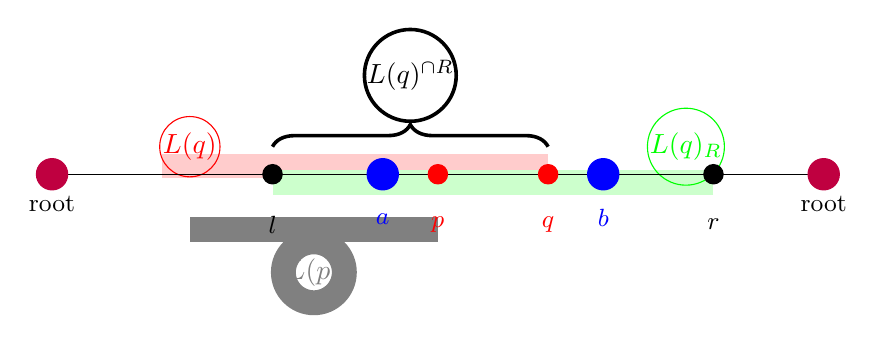
\begin{tikzpicture}[scale=\scale]
	\draw [decorate,line width=1.3pt, decoration = {brace,mirror,amplitude=8pt}] (9,0.5) --node [above=0.3cm] {$L(q)^{\cap R}$}  (4,0.5);
		\draw [color=red!20,line width=9pt]	(9,0.15) -- (2,0.15);
		\draw [color=green!20,line width=9pt] (12,-0.15) -- (4,-0.15);
		\draw [color=gray,line width=9pt] (7,-1) -- node[below] {$L(p)$} (2.5,-1);
		\node [color=red] at (2.5,0.5) () {$L(q)$};
		\node [color=green] at (11.5,0.5) () {$L(q)_R$};
		\draw [color=black] (0,0) -- (14,0);
		\foreach \i in {0, 14}
			\node [color=purple,inner sep=4,label={[yshift=-0.9cm]\small root},circle,fill] at (\i,0) () {};
		\foreach \i/\c/\l/\is in {4/black/l/2, 6/blue/a/4, 7/red/p/2, 9/red/q/2, 10/blue/b/4, 12/black/r/2}
			\node [fill,circle,inner sep=\is,label={[yshift=-0.9cm,color=\c]\small $\l$},color=\c] at (\i,0) () {};
	\end{tikzpicture}
	\caption{\small  Since the left endpoint of $L(p)_R$ is  $l$, the left endpoint of $L(p)$ is to the left of $l$. Therefore, $L(p)$ crosses $L(q)^{\cap R}$ on left and it is a candidate for $L^*(q)$. Therefore, $L(p)\cap L(q)^{\cap R}\subseteq L^*(q)\cap L(q)^{\cap R}$ and we have $a\in L^*(q)\cap L(q)^{\cap R}$. But then, $e\notin E^(B^\rightarrow(q))$. Contradiction!.}
	\label{fig:atmost2finalcont}
\end{figure}



\subsection{Overview of proof of \cref{thm:informalmain} -- no inside atoms}
\label{sec:noinside}

%Let \hyperlink{tar:G=(V,E,x)}{$G=(V,E,x)$} be an undirected graph equipped with a weight function $x:E\to\R_{\geq 0}$ (the solution to \cref{eq:tsplp}) such that for any cut $(S,\overline{S})$ such that $u_0,v_0\not\in S$, $x(\delta(S))\geq 2$.
%For some (small) $\eta\geq 0$, consider a single  connected component ${\cal C}$ of \hyperlink{tar:crossing}{crossing} \hyperlink{tar:nearmincut}{$\eta$-near min cuts} of $G$.  Given ${\cal C}$ we can partition vertices of $G$ into sets $a_0,\dots,a_{m-1}$ (called atoms); this is the coarsest partition such that for each $a_i$, and each $(S,\overline{S})\in {\cal C}$, we have $a_i\subseteq S$ or $a_i\subseteq \overline{S}$.  One of these atoms,  $a_0$ is the atom that contains $u_0,v_0$. We call $a_0$ the {\em root}.
Given a connected component $\C$ of cuts in $\cN_\eta$, we can partition vertices of $G$ into sets $a_0,\dots,a_{m-1}$ (called atoms); this is the coarsest partition such that for each $a_i$, and each $(S,\overline{S})\in {\cal C}$, we have $a_i\subseteq S$ or $a_i\subseteq \overline{S}$.  One of these atoms,  $a_0$ is the atom that contains $u_0,v_0$. We call $a_0$ the {\em root}.  \textit{In the following, we will often identify an atom with the set of vertices that it represents}\footnote{For example, it will be convenient to write cuts as subsets of atoms. In this case the cut is the union of the vertices in those atoms.}.

If $\eta=0$, then  \cite{DKL76}) shows that the structure of cuts in $\C$ can be represented by a cycle; namely we can arrange these atoms around a cycle such that, perhaps after renaming, for any $0\leq i\leq m-1$, $x(E(a_i,a_{i+1 \text{ mod } m}))=1$ and cuts of $\C$ are just the mincuts of this cycle.

%{\em cactus structure}  then we can arrange the $a_i$'s of a connected component around a cycle, say $a_1,\dots,a_m$ (after renaming), such that $x(E(a_i,a_{i+1}))=1$ for all $i$.
As mentioned, \cite{Ben95,BG08} studied the case when $0 <\eta\leq 2/5$ and introduced the notion of {\em polygon representation}, in which case atoms can be placed on the sides of an equilateral polygon $P$ and some atoms  placed inside  the polygon, such that every cut in ${\cal C}$ can be represented by a diagonal of this polygon. See \autoref{fig:polygonrepresentation}. %Later, \cite{OSS11} studied the structure of edges of $G$ in this polygon when $\eta<1/100$.

{\em In the rest of this section, we fix $\C$ and we outline the ideas behind the proof of \cref{thm:informalmain} in the special case that the polygon $P$ representing the connected component of cuts $\C$ contains  no inside atoms}. This latter assumption simplifies the argument but still illustrates many of the main ideas. 
%As in the case of a cactus, 

We assume that the atoms of $P$ are labelled counterclockwise from $a_0$ to $a_{m-1}$. We associate to each diagonal (defining a cut) the side which does not contain $a_0$.\footnote{The reason we do this is that it is crucial for subsequent arguments to be able to condition on near min cuts being trees using \cref{lem:treeconditioning}, i.e., that for $S$ a near min cut, $E(S) \cap T$ is very likely to be a tree. However, this lemma can only be used on sets which do not contain $u_0,v_0$.} Thus, we will refer to a cut by the set of outside atoms it contains, say $[a_i,a_j]$, $i < j$. (This denotes the side of the diagonal containing the atoms $a_i, a_{i+1}, \ldots, a_j$.) We equivalently refer to this cut by giving the left and right polygon points of its diagonal $[p_{i-1},p_j]$.

As mentioned above, the raison d'etre for the slack vector $s^*$  that we construct here is to restore the feasibility of cuts $S$ in $\cC_2$ which are odd in the tree but which have $s_e$ negative on some edges in $\delta(S)$.  The high level approach in the proof is the following. Initialize $s_e^*:= 0$ for all $e$. Now define a set of {\em bad events} whose occurrence signifies that some  of these near min cuts are potentially in need of such a repair. These bad events should satisfy the follow desiderata:
\begin{itemize}
\item[(a)] Each bad event occurs with probability $O(\eta)$, where the probability is taken over the choice of tree $T$.
\item [(b)]  The occurrence of a bad event $B$ in a tree $T$ triggers a {\em slack increase} on an associated set of edges $E(B)$. Specifically, when $B$ occurs, each edge $e \in E(B)$  has its slack $s_e^*$ increased by $\alpha x_e$. 
\item [(c)] Each edge $e$  is in $E(B)$ for a {\em constant number of bad events} $B$. Combining (a) and (b), this implies that $\E{s_e^*} = O(\eta\alpha x_e)$ (condition 2 of \cref{thm:informalmain}).% since $\E{s_e^*}$ is the increase $O(\eta x_e)$ times the probability that one of $e$'s bad events occurs.
\item[(d)] Each $\eta$-near-min cut $S$ is associated with a constant number of bad events ${\mathcal B}(S)$, such that when $\delta(S)_T$ is odd, at least one of the bad events $B \in {\mathcal B}(S)$ occurs. We will ensure that the edges in $E(B)$ (on which slack increases are triggered) are a subset of $\delta(S)$ of fractional value at least   $\Omega(1)$. Therefore, if $S$ is odd in the tree, $s^*_T(\delta(S)) \ge \alpha x(E(B)) \ge \Omega(\alpha)$ implying condition (iii) of \cref{thm:informalmain} (once the constant  are chosen appropriately).


\end{itemize}

\subsection{Satisfying the above desiderata}
Consider any near min cut $S$ in $P$, which is crossed on the left and on the right (see \cref{def:SLR} for the definition of being crossed on left/right) .  Let $S_L$ and $S_R$ be the cuts crossing $S$ on the left and right {\em with minimum sized intersection} with $S$. See \autoref{fig:S-SR-SL}.





One of the very nice things about cuts crossed on both sides is the following:

\begin{claim}\label{claim:C2evenwhp}
For any near min cut $S \in \cC_2$, $\P{\delta(S)_T= 2} \ge 1-O(\eta)$.
\end{claim}
\begin{proof}[Proof sketch]
To see this, for a set $S$ crossed on both sides, let
$$E^{\leftarrow} (S) := E(S\cap S_L, S_L \smallsetminus S), \quad E^{\rightarrow} (S) := E(S\cap S_R, S_R\smallsetminus S),\quad E^\circ(S) := \delta(S) \smallsetminus E^{\leftarrow} (S) \smallsetminus E^{\rightarrow} (S)$$
and consider the bad events
\begin{equation}\label{eqn:badfirst} B^\leftarrow(S) := \mathbb{1}\{E^{\leftarrow} (S)_T\ne 1\}\quad B^\rightarrow(S)=\mathbb{1}\{E^{\rightarrow} (S)_T\ne 1\}\quad B^\circ(S):= \mathbb{1}\{E^\circ (S)_T\ne 0\}.	
\end{equation}
 See \autoref{fig:S-SR-SL}. 

Clearly if none of these bad events occur, then $S$ is even in the tree (i.e., $\delta(S)_T = 2$).
Now, note that $S, S_R, S_L$ are all $\eta$-near min cuts and so by \cref{lem:nmcuts_largeedges} and \cref{lem:treeoneedge}, we have $x(E^\leftarrow (S)) \ge  1-\eta/2$, $x(E^\rightarrow (S)) \ge  1-\eta/2$, $x(E^\circ(S)) = x(\delta (S)\smallsetminus E^\leftarrow (S)\smallsetminus E^\rightarrow (S)) = O(\eta)$ and $\P{B^\leftarrow(S)}, \P{B^\rightarrow(S)}, \P{B^\circ(S)} = O(\eta).$
\end{proof}


The next step in our plan is to decide what slack increases are triggered by these bad events. The first thing one might think of is to have the above bad events  (\ref{eqn:badfirst}) trigger a slack increase on $E^\leftarrow (S) \cup E^\rightarrow (S)$. Namely, for each set $S$ crossed on both sides:
$$\forall e \in  E^\leftarrow (S) \cup E^\rightarrow (S)\quad \text{ set }s^*_e :=
 	\alpha x_e \cdot \mathbb{1}\{\text{at least one of } B^\leftarrow(S), ~B^\rightarrow(S) \text{ or } B^\circ(S)\text{ occurs}\}.$$
 	In addition to desiderata (a) and (b), this approach satisfies (d) since $x(E^\leftarrow (S) \cup E^\rightarrow (S))\ge 2-\eta$.
 
 Unfortunately though, this  does not satisfy desiderata (c), since if $e \in E(a_i, a_j)$, it could be that $e \in  E^\leftarrow (S) \cup E^\rightarrow (S)$ for {\em many} near min cuts $S$ %with one endpoint in between $a_i$ and $a_j$, 
     in which case  $$\E{s^*_e} = \alpha x_e \cdot\P{\exists S\text{ odd in }T\text{ s.t. }e \in E^\leftarrow (S) \cup E^\rightarrow (S))}$$ could be way too large (say, around $\alpha x_e$). 
  

So, rather than defining a bad event for every cut $S$ crossed on both sides individually (i.e., up to $O(m^2)$ events), we instead define a constant number of bad events for each polygon point $p$, hence at most $O(m)$ events. 


\subsubsection{Defining bad events for each polygon point}

For a fixed polygon point $p$, 
let $L := L(p)$ be the set crossed on both sides that extends farthest clockwise from $p$ and as above, let $L_R$ be the cut that crosses it on the right with the minimum number of outside atoms in the intersection.  Analogously define $R:= R(p)$ and $R_L$. See \autoref{fig:LpRp}.


Now we consider two bad events: 
\begin{equation}
\label{defn:badevents}
\begin{aligned}
	B^\rightarrow (p) &= \mathbb{1}\{E^{\rightarrow} (L(p))_T\ne 1\text{ or }E^\circ (L(p))_T\ne 0\}%\notag
	\\
B^\leftarrow (p) &= \mathbb{1}\{E^{\leftarrow} (R(p))_T\ne 1\text{ or }E^\circ (R(p))_T\ne 0\}. 
\end{aligned}
\end{equation}

For these events, we have the following two claims:
\begin{claim}\label{claim:1}
	 For any near min cut $S=[p,q]$, $E^{\rightarrow} (L(q)) = E^\rightarrow (S)$ and $E^{\leftarrow} (R(p)) = E^\leftarrow (S)$. Moreover, $E^\circ (S) \subset E^\circ (L(p))\cup E^0 (R(p)$. See \autoref{fig:ErL=ErS}. Therefore, if neither $B^\rightarrow (q)$ or $B^\leftarrow (p)$ occur, then $\delta(S)_T$ is even.  
\end{claim}


In addition we have
\begin{claim}\label{claim:2}
	 For any polygon point $p$, $\P{B^\rightarrow (p)}, \P{B^\leftarrow (p)} = O(\eta)$.
\end{claim}
This follows arguments similar to those used in \cref{claim:C2evenwhp}, using that $x(E^\rightarrow (L(p)))\ge 1- \eta/2$, and $x(E^\circ (L(p)) = O(\eta)$ (and similarly for $R(p)$).

%Now suppose that $S=[q,p]$ (so the rightmost outside atom of $S$ is immediately to the left of $p$). Then $E^\rightarrow (S) = E^\rightarrow (L(p))$, since $S_R = L_R$ as shown in Figure ??.

%Moreover, by the argument above, $x(E^\rightarrow (L(p)))\ge 1- \eta/2$, and $x(E^\circ (L(p)) = O(\eta)$, and so, as above, we could define corresponding bad events for which
%$$\P{B^\rightarrow(L(p))\text{ or } B^\circ (L(p))} = O(\eta).$$ 
 
 These bad events satisfy the desiderata (a) and (d) (assuming we define $E(B)$ such that $x(E(B)) \in  \Omega(1)$). 
 
\subsubsection{Defining the slack increase sets for bad events} 

It remains to determine the sets $E(B^\rightarrow(p)),E(B^\leftarrow(p))$  for which slack increases are triggered when the bad events occur. In particular, we will let $E(B^\rightarrow(p)) \subseteq E^\rightarrow(L(p))$ and $E(B^\leftarrow(p)) \subseteq E^\leftarrow(R(p))$ such that:
\begin{enumerate}
\item[(*)] $x(E(B^\rightarrow(p))) \ge \Omega(1)$ and $x(E(B^\leftarrow(p))) \ge \Omega(1)$ (to guarantee (d)),
\item[(**)] All edges $e$ are in at most a constant number of sets $E(B)$ (to guarantee (c)). 
\end{enumerate}
Assuming we can satisfy (*) and (**), we can set $s^*_e = \alpha x_e$ for all $e \in E(B)$ when $B$ occurs to satisfy all four desiderata.

\paragraph{First try:} The most natural choice is to simply let $E(B^\rightarrow(p)) = E^\rightarrow (L(p))$. Here, (*) obviously holds but unfortunately (**) fails. 
%That is, 
%$$\forall e \in  E^\rightarrow (L(p) ) \text{ set }s^*(e) := 
 	%\eta x_e \cdot \mathbb{1}\{B^\rightarrow(p)  \text{ or } B^\circ(p)\text{ occur}\}.$$
 	%We might call this a {\em "right" slack increase for polygon point $p$}, triggered by the bad event $B^\rightarrow(p)  \text{ or } B^0(p)$ and we can define a "left" slack increase  similarly for each polygon point.) 
 	Indeed, there are examples (see \autoref{fig:einmanyL(p)}) for which there exist edges $e\in E(a_i,a_j)$ with $|j-i|=\Omega(m)$ that belong to 
 	$E^\rightarrow(L(p_k))$ for $\Omega(m)$ many values of $i\leq k\leq j$.


\paragraph{Second try:} 
Let $a_i$ be the atom immediately to the left of $p$ and $a_{i+1}$ the atom immediately to the right of $p$ (i.e. $p=p_i$). Note that all edges with one endpoint in $a_i$ and one in $a_{i+1}$ are in $E^\rightarrow (L(p))$. Now if it was always the case that $x(E(a_i, a_{i+1}))\geq \gamma$ for some universal constant $\gamma > 0$, then, when one of these bad events occurs, say $B^\rightarrow(p)$, we could simply increase the slack of every edge $e$ in $E(a_i, a_{i+1})$ by $\alpha x_e$. 
This approach is analogous to the method employed in \cite{KKO21} where slack was increased on OPT edges. One might have some hope that this is true since it holds with $\gamma = 1$ for the cactus representation of min cuts (i.e. when $\eta = 0$). 

Unfortunately, as observed in \cite{OSS11} there is a family of near minimum cuts such that the polygon representation has no inside atoms, yet $E(a_i,a_{i+1})=\emptyset$ for some consecutive pairs of (outside) atoms (see \autoref{fig:nearmincutbadexample}) (even though there are cuts whose diagonals end between those atoms). So, this method is doomed even if inside atoms are not present.

\paragraph{Our method:} 
The first try works if there are no ``long'' edges. So, to rectify that attempt we essentially ``ignore'' long edges (edges between distant atoms) in our charging argument and argue that they only contribute minimally to $E^\rightarrow(L(p))$ and $E^\leftarrow(R(p))$. 

%However, we redefine the edges on which slack is increased in response to these bad events to ensure that each edge has at most a constant number of bad events that can cause its slack to increase. 
To this end, define $L(p)^{\cap R} := L(p) \cap L(p)_R$, and let $L^*(p)$ be the cut crossing $L(p)^{\cap R}$ on the left that {\em maximizes} the number of outside atoms in the intersection of $L^*(p)$ and $L(p)^{\cap R}$ (and similarly $R^*(p)$ to maximize the intersection with $R(p)^{\cap L}$ on the right). If $L^*(p)$ does not exist, i.e. no cut crosses $L(p)^{\cap R}$ on the left, set $L^*(p) = \emptyset$, and similarly for $R^*(p)$. See  \autoref{fig:L*R*}. We let:
\begin{equation}
\begin{aligned}
	E(B^\rightarrow (p)) &:= E( L(p)^{\cap R} \smallsetminus L^*(p), L(p)_R \smallsetminus  L(p)^{\cap R})  \\
	E(B^\leftarrow (p)) &:= E( R(p)^{\cap L} \smallsetminus R^*(p), R(p)_L \smallsetminus  R(p)^{\cap L}).
\end{aligned}
\label{defn:slackincrease}
\end{equation}



%and have the bad events trigger slack increases for each polygon point $p$ as follows:
%\begin{align*}
%	\forall e\in  E(B^\rightarrow (p))~~s^*(e)&:= \eta x_e \cdot \mathbb{1}\{ B^\rightarrow (p)\text{ occurs}\}\quad\text{ and }\\
%\forall e\in  E(B^\leftarrow (p))~~s^*(e)&:= \eta x_e \cdot \mathbb{1}\{ B^\leftarrow (p)\text{ occurs.}\}\end{align*}
%With these criteria for slack increases, since edges in $E(B^\rightarrow (p))$ (and similarly $E(B^\leftarrow (p))$) have endpoints that are in $2\eta$-NMCs (See Figure ??), we still have:

The following claim establishes (*) for \cref{defn:slackincrease}. It can be proved using methods similar to \cref{claim:C2evenwhp}; see \autoref{fig:ErL=ErS}.
\begin{claim}\label{claim:xvaluenoinside}
	For all polygon points $p$, $x(E(B^\rightarrow (p))), x(E(B^\rightarrow (p)))\ge 1-O(\eta)$.
\end{claim}

And finally, the following claim establishes (**):

\begin{claim}\label{claim:atmost2sets}
	For any edge $e$, we have $e\in E(B^\rightarrow (p))$ for at most one polygon point $p$ and similarly  $e\in E(B^\leftarrow (q))$ for at most one polygon point $q$.
\end{claim}

The proof of \cref{claim:atmost2sets} is more involved. For an outline of the arguments used, see Figures \ref{fig:locl'r'circ}, \ref{fig:locl'r'}, \ref{fig:l'notR}, \ref{fig:l'notL}, \ref{fig:atmost2finalcont}.

%\begin{figure}[htb]\centering
	
%\end{figure}



%\begin{figure}[htb]\centering
%	\end{figure}

%\begin{figure}[htb]\centering
	
%\end{figure}





%\begin{figure}[htb]\centering
	
%\end{figure}


%\vspace{0.2in}
%Putting it all together, the definitions satisfy all four desiderata.
%
%\begin{itemize}
%\item[(a)] Each bad event occurs with probability $O(\eta)$  (Claim 2).
%\item [(b)] Each edge $e$  is associated with a constant number of bad events such that, when one of the associated bad events occurs, the slack  $s_e^*$ is increased by $\eta x_e$ (Claim 4). Again, we note that (a) and (b) immediately imply that $\E{s_e^*} = O(\eta^2 x_e)$, condition 2 of \cref{thm:informalmain} (since $\E{s_e^*}$ is the increase $\eta x_e$ times the probability that one of $e$'s bad events occurs).
%\item [(c)] Each cut $S\in C(\eta)$ is associated with a constant number of bad events $\mathcal B(S)$ such that 
%$S$ is odd in the tree only if at least one of the bad events in  $\mathcal B (S)$ occurs (Claim 1).
%\item[(d)] 	The edges that are increased when a bad event in $\mathcal B (S)$ occurs are a subset of $\delta(S)$ and have fractional value at least   $1-O(\eta)$ (by Claims 1 and 3). This implies condition 3 of \cref{thm:informalmain}.
%\end{itemize}
%Thus, we have shown how to prove \cref{thm:informalmain} in the special case that the polygon has no inside atoms. For a more formal version of the arguments in this section, see Appendix ??.


\subsection{Extending to polygons with inside atoms}

For the general case, we still follow the same proof outline satisfying the four desiderata using the same definition of bad events given in (\ref{defn:badevents}) and the same definition of edges on which slack is increased in response to bad events given in (\ref{defn:slackincrease}).

We need to address the following challenges when generalizing the above proof:
\begin{enumerate}[(1)]
\item Edges may have endpoints adjacent to inside atoms. The proof outline above crucially used that both endpoints of every edge were outside atoms. 
\item Regions of the polygon we could previously assume were empty may now contain inside atoms.
\item While the sets are still defined such that they do not contain the root, the root (i.e., the atom containing $\{u_0, v_0\}$) is no longer necessarily an outside atom. 
Therefore we can have a sequence of cuts not containing the root wrapping around the polygon such that each cut crosses the one before it. In this case, the notion of ``left" and ``right" becomes unclear. One can still define ``left" and ``right" synonymously with clockwise and counterclockwise, but we can no longer say that an outside atom is to the left (and not to the right of) another outside atom, nor can we collapse the diagonals of the polygon to intervals of a line. 
\end{enumerate}
To handle these complexities, we introduce additional structural properties of polygons with inside atoms. These are presented in \autoref{sec:polygonsnewproperties}.

